\chapter{Genauer Vergleich}

In diesem Kapitel werden die vorher ausgewählten Suchmaschinen genauer verglichen. Dafür werden alle vier Suchmaschinen aufgesetzt und getestet. Hier wird Wert auf alle Aspekte des Prozesses gesetzt. Da ich dieses Projekt nicht nach meiner Bachelor-Arbeit wohl nicht weiter verfolgen kann, ist es auch wichtig zu schauen, wie leicht ein neuer Administrator sich in das System einlernen kann, beziehungsweise wie leicht das System zu verstehen und administrieren ist. Deshalb wird auch die Dokumentation verglichen und geschaut, wie groß die Community der einzelnen Suchmaschinen ist. Die genaueren Kriterien werden nun im Folgenden mit Erklärungen aufgeführt. Da es nicht für jede der Suchmaschinen ein offizielles Docker-Image gibt, werden der Fairness halber alle Systeme manuell aufgesetzt.

Das Test-System hat folgende Spezifikationen:

\begin{itemize}
    \item CPU: 4 Kerne
    \item RAM: 16 Gigabyte
    \item Festplattenspeicher: 20 GB
    \item Betriebssystem: Ubuntu 18.04.03 LTS
\end{itemize} 

Auf das System wird daraufhin die MySQL Datenbank von Dietrich-Online Projekt aufgespielt. Dies für diesen Vergleich die einzige Datenquelle sein.

\section{Aufbau der Tests}

\subsection{Installation}

Im ersten Schritt wird die Installation bewertet, dabei wird geschaut, wie einfach es ist die Software zu installieren. Hierbei ist es wichtig zu schauen, wie simpel die Installation ist. Existiert zum Beispiel ein Installations-Wizard? Wie viel muss manuell in den Dateien geändert werden? Müssen viel externe Programme nachinstalliert werden?

\subsection{Oberfläche}

Als Nächstes folgt der Ersteindruck der Software und Oberfläche. Dabei wird geschaut, wie übersichtlich die Oberfläche ist, falls eine gegeben ist, und wie verständlich das System für Einsteiger ist. Dafür wird im ersten Schritt möglichst auf die Dokumentation verzichtet, um einen Ersteindruck zu liefern, wie gut die Oberfläche für sich selbst spricht. Dies dient dazu um, zu schauen wie der neue Administrator bestimmte Aufgaben ohne Vorkenntnisse erfüllen kann. Besondere Punkte dabei sind zum Beispiel: Wie viel kann man über die Oberfläche konfigurieren? Lassen sich Updates direkt über die Oberfläche einspielen? Ist die Seite responsive? Wie funktioniert die Nutzerverwaltung?

\subsection{Indexierung}

Hier geht es darum festzustellen, wie einfach eine Indexierung der einzelnen Dateien möglich ist. Darunter fällt zum Beispiel: Kann man die Daten über die grafische Benutzeroberfläche indexieren lassen? Kann man das System darauf anweisen Änderungen direkt neu zu indexieren?


\subsection{Dokumentation}

Im dritten Schritt wird die Dokumentation analysiert. Hierbei wird das Augenmerk auf die Übersichtlichkeit und Verständlichkeit gelegt. Auch hier ist es wieder wichtig zu schauen, ob die Dokumentation auch ohne Vorkenntnisse gut zu verstehen ist. Da in diesen Kurztest nicht alle Funktionen durchgetestet werden können, ist es leider auch nicht möglich zu schauen, ob alle Funktionen korrekt und ausführlich dokumentiert sind. Sollte allerdings schon von den Grundfunktionen eine schlechte oder fehlende Dokumentation auffallen wird dies natürlich erwähnt. 

\subsection{Absetzen einer Anfrage und Integration in PHP}

Im letzten Schritt werden eine Query abgesetzt. Dabei wird in PHP die Zeit gemessen, die für eine solche Abfrage benötigt wird.

Die dabei verwendete Query ist einer der bisher am langsamsten laufenden Query’s. Er ermittelt alle Lemmata vom Buchstaben S und baut alle Daten, die zur Anzeige benötigt werden zusammen \ref{img:lAdminSample}. Die Tabellen die für diese Ansicht gebraucht werden, sind in diesen Diagramm \ref{img:lAdminStructure} zu finden. Eigentlich muss man sagen, dass es sich hierbei nicht um einen Query handelt, sondern um zwei. Der erste Sammelt alle ID’s aus der Datenbank, welche unter dem Buchstaben zu finden sind:

\begin{figure}
	\centering
	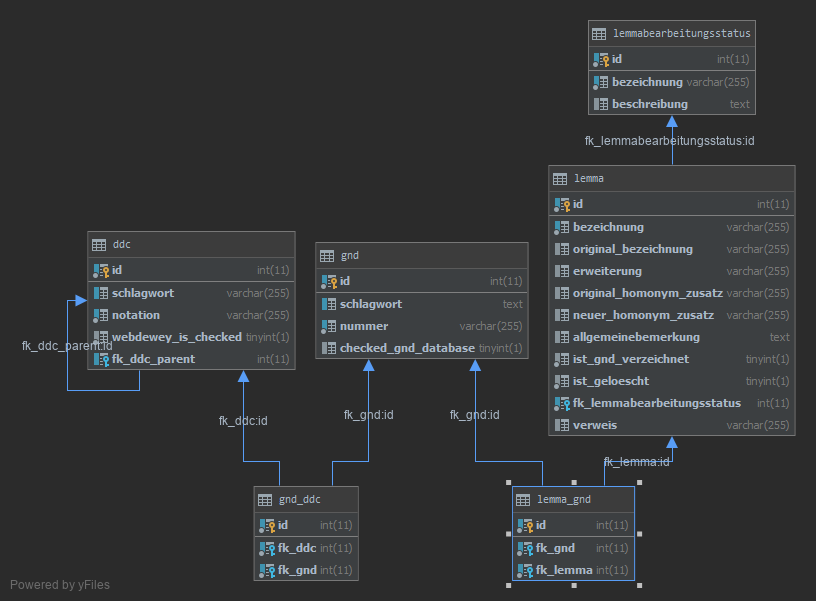
\includegraphics[width=0.8\linewidth]{images/structure_lemmaadministration.png}
	\caption{Tabellenaufbau der Lemma-Administration Übersicht.}
	\label{img:lAdminStructure}
\end{figure}

\begin{figure}
	\centering
	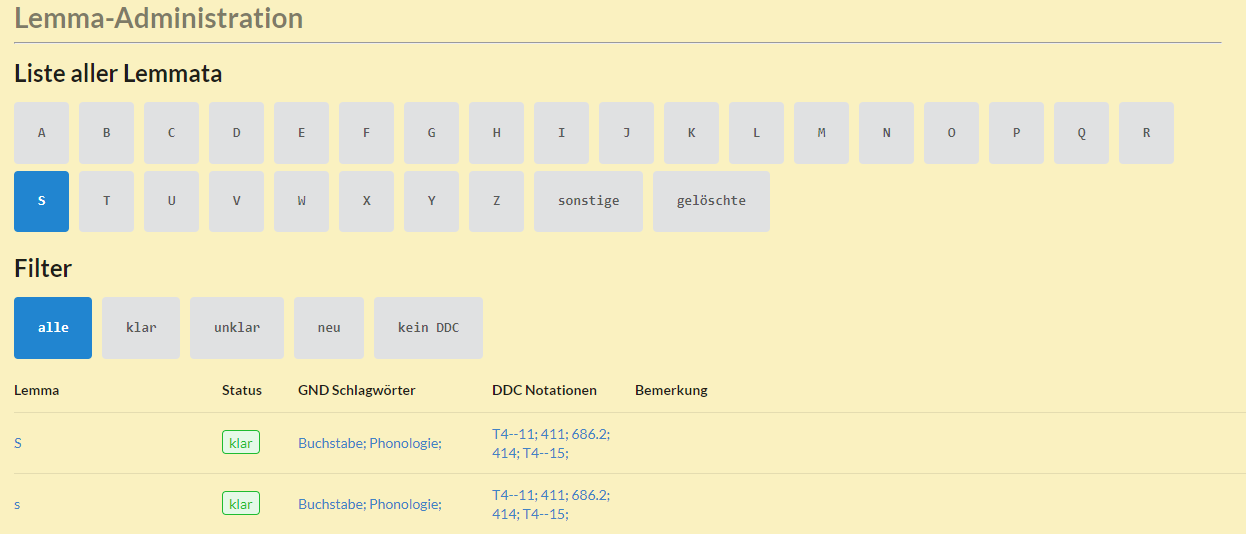
\includegraphics[width=1\linewidth]{images/lemmaadministration_sample.PNG}
	\caption{Frontend Ansicht der Lemma-Administration mit geladenen Buchstaben S (Ausschnitt).}
	\label{img:lAdminSample}
\end{figure}

\lstset{language=SQL}
\begin{lstlisting}[frame=single] 
    SELECT
    lemma.id
FROM lemma
WHERE
    lemma.bezeichnung LIKE 'S%'
    AND lemma.ist_geloescht = 0
ORDER BY
    lemma.bezeichnung ASC,
    lemma.id ASC;
\end{lstlisting}

Im zweiten Schritt werden dann die gerade geholten ID’s mit vielen JOIN’s für die Darstellung vorbereitet.

\lstset{language=SQL}
\begin{lstlisting}[frame=single] 
SELECT  lemma.id,                        
        [...] #Lemma, GND und DCC-Spalten        
FROM lemma lemma
      
INNER JOIN lemmabearbeitungsstatus lemmaBStatus
ON lemma.fk_lemmabearbeitungsstatus = lemmaBStatus.id

LEFT JOIN lemma_gnd lemma_gnd_map ON lemma.id = lemma_gnd_map.fk_lemma
LEFT JOIN gnd gnd ON lemma_gnd_map.fk_gnd = gnd.id
LEFT JOIN gnd_ddc gnd_ddc_map ON gnd.id = gnd_ddc_map.fk_gnd
LEFT JOIN ddc ddc ON gnd_ddc_map.fk_ddc = ddc.id
WHERE lemma.id IN ([Array of Lemma IDs])
ORDER BY lemma.bezeichnung ASC, lemma.id ASC;

\end{lstlisting}

\subsection{Vorbereitung}

Vor der Serverübergabe wurden nur ein paar Hilfsprogramme, wie VIM und Curl installiert. Als Datenbank habe ich dann noch eine MariaDB Instanz aufgesetzt, welche ein aktuelles Datenbank-Abbild von Dietrich-Online erhalten hat.